\documentclass[10pt,a4paper]{report}

\usepackage[utf8]{inputenc}
\usepackage{amsmath}
\usepackage{amsfonts}
\usepackage{amssymb}
\usepackage{graphicx}
\usepackage{color}
\usepackage{enumitem}
\usepackage[top=1cm, bottom=2cm, left=2cm, right=2cm]{geometry}

\usepackage{fancyhdr}
\pagestyle{fancy}

\fancyhead{}
\fancyfoot{} 
\lhead{ \hspace{0.1cm} Promo 2014-2015  \hspace{0.4cm} \vline}
\chead{Advanced Algorithm}
\rhead{K.B - K.L - N.R}
\rfoot{\thepage}

\author{Kevin BASCOL, Kevin LAOUSSING, Nicolas REYNAUD}
\title{Algorithme avancé : \\Problème du voyageur de commerce}

\makeatletter
\renewcommand{\thesection}{\@arabic\c@section}
\makeatother

\begin{document}

\makeatletter
	\begin{titlepage}
	
	\begin{figure}
		\begin{minipage}[c]{.46\linewidth}
		\end{minipage} \hfill
		\begin{minipage}[c]{.20\linewidth}

		\end{minipage}
	\vspace{1cm}
	\end{figure}
	
	\centering
		{
		\hrule height 2pt
		\vspace{0.7cm}
		\Huge \textbf{\@title}}\\
		\vspace{0.7cm}
		\hrule height 2pt
		
		\vfill
		\vspace{1cm}
		\@author\\
		\end{titlepage}
\makeatother
\setcounter{secnumdepth}{5}
\setcounter{tocdepth}{5}
\renewcommand{\contentsname}{Sommaire}
\begingroup\makeatletter
\def\@makeschapterhead#1{%
  {\parindent \z@ \raggedright
    \normalfont
    \interlinepenalty\@M
    \Huge \bfseries  #1\par\nobreak
    \vskip 20pt% <---- à réduire pour avoir plus de place
  }}\makeatother
\tableofcontents
\endgroup
\thispagestyle{empty}
\setcounter{page}{0}
\newpage

\newgeometry{top=2cm, bottom=2cm, left=2cm, right=2cm}

\section{Introduction}
\begin{flushleft}
Le problème du voyageur de commerce, consiste en la recherche d'un trajet minimal permettant à un voyageur de visiter n villes. En règle générale on cherche à minimiser le temps de parcours total ou la distance totale parcourue.\\
Il existe plusieurs approche pour résoudre ce problème, parmi lesquelles on peut distinguer les approches donnant des résultats exactes et les approches donnant des résultats approximatives.
L'objectif de notre projet est d'implémenter ces différentes approches, de pouvoir les tester, de pouvoir analyser les résultats et de déterminer quel est le meilleur compromis entre temps de résolutions et "exactitude" de la solution.
\end{flushleft}


\section{Organisation du projet}

	\subsection{Planning}
	
		\subsubsection{Diagramme de gantt}
		
			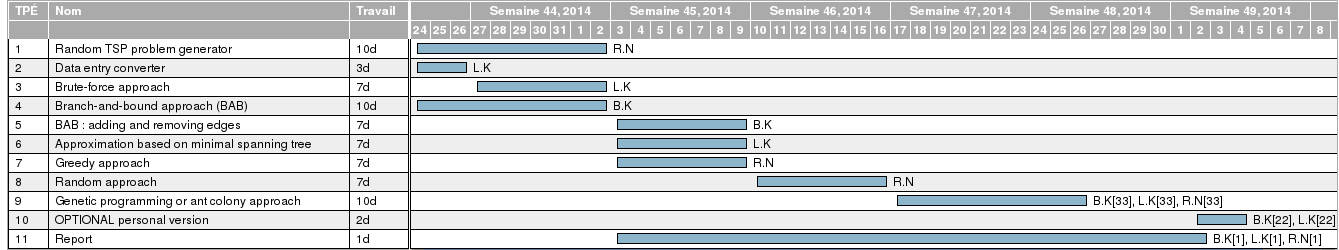
\includegraphics[scale=0.37]{./Ressource/planning_AA.png}
		
	
	\subsection{Langage utilisé et outil de développement}
	
\section{Algorithmes de résolution de problème du voyageur de commerce}

	\subsection{Structure de donnée}
	
	\subsection{Algorithme donnant une solution optimale}
		\subsubsection{Brute force}
		
		\subsubsection{Séparation et évaluation}	
		
		\subsubsection{Séparation et évaluation avec utilisation de matrice}	
		
	\subsection{Algorithme donnant une solution approximative}
	
		\subsubsection{Approche gloutonne}
		
		\subsubsection{Approche aléatoire}
		
		\subsubsection{Approche avec l'arbre couvrant de poids minimal}
		
		\subsubsection{Approche génétique}
		
\section{Etudes d'efficacités des algorithme}

	\subsection{Tests effectués}
	
	\subsection{Observations}
	
	\subsection{Conclusion}

\section{Programmes annexes}

	\subsection{DataConverter}
	
	\subsection{TSPGenerateur}
	
\section{Conclusion}
	





\end{document}